%\documentclass[25pt, a0paper, landscape]{tikzposter}
\documentclass[25pt, a0paper]{tikzposter}
\tikzposterlatexaffectionproofoff
\usepackage[utf8]{inputenc}
\usepackage{authblk}
\usepackage{cite}
\makeatletter
\renewcommand\maketitle{\AB@maketitle} % revert \maketitle to its old definition
\renewcommand\AB@affilsepx{\quad\protect\Affilfont} % put affiliations into one line
\makeatother
\renewcommand\Affilfont{\Large} % set font for affiliations
\usepackage{amsmath, amsfonts, amssymb}
\usepackage{tikz}
\usepackage{pgfplots}
% align columns of tikzposter; needs two compilations
\usepackage[colalign]{column_aligned}
\usepackage{graphics}
\RequirePackage[nottoc]{tocbibind}


\def\kk{KicKinect}
\def\kki{\textit{\kk}}
\def\linearBlendSkinning{\textit{\linearBlendSkinning}}
\def\linearBlendSkinningn{Linear Blend Skinning}
\def\lbs{\textit{LBS}}
\def\kinectSDK{\textit{\kinect{} SDK}}
\def\kinect{\textit{Kinect}}

\newcommand{\image}[3]{
	\begin{center}
		\includegraphics[width=#3]{#1}
		\
		\begin{flushleft}
			\begin{center}
				\textit{#2}
			\end{center}
		\end{flushleft}
	\end{center}
}
% tikzposter meta settings
\usetheme{Default}
\usetitlestyle{Default}
\useblockstyle{Default}

%%%%%%%%%%% redefine title matter to include one logo on each side of the title; adjust with \LogoSep
\makeatletter
\newcommand\insertlogoi[2][]{\def\@insertlogoi{\includegraphics[#1]{#2}}}
\newcommand\insertlogoii[2][]{\def\@insertlogoii{\includegraphics[#1]{#2}}}
\newlength\LogoSep
%\setlength\LogoSep{-70pt}
\setlength\LogoSep{-160pt}

\renewcommand\maketitle[1][]{  % #1 keys
    \normalsize
    \setkeys{title}{#1}
    % Title dummy to get title height
    \node[inner sep=\TP@titleinnersep, line width=\TP@titlelinewidth, anchor=north, minimum width=\TP@visibletextwidth-2\TP@titleinnersep]
     (TP@title) at ($(-0.5\textwidth+44pt+0.5\titlewidth, 0.5\textheight-\TP@titletotopverticalspace)$) {\parbox{\TP@titlewidth-2\TP@titleinnersep}{\TP@maketitle}};
   % (TP@title) at ($(0, 0.5\textheight-\TP@titletotopverticalspace)$) {\parbox{\TP@titlewidth-2\TP@titleinnersep}{\TP@maketitle}};
    \draw let \p1 = ($(TP@title.north)-(TP@title.south)$) in node {
        \setlength{\TP@titleheight}{\y1}
        \setlength{\titleheight}{\y1}
        \global\TP@titleheight=\TP@titleheight
        \global\titleheight=\titleheight
    };

    % Compute title position
    %\setlength{\titleposleft}{-0.5\titlewidth}
    \setlength{\titleposleft}{-0.5\textwidth+44pt}
    \setlength{\titleposright}{\titleposleft+\titlewidth}
    \setlength{\titlepostop}{0.5\textheight-\TP@titletotopverticalspace}
    \setlength{\titleposbottom}{\titlepostop-\titleheight}

    % Title style (background)
    \TP@titlestyle

    % Title node
    \node[inner sep=\TP@titleinnersep, line width=\TP@titlelinewidth,
    anchor=north, minimum width=\TP@visibletextwidth-2\TP@titleinnersep]
    at (\titleposleft+0.5\titlewidth,0.5\textheight-\TP@titletotopverticalspace)
     %anchor=north, minimum width=\TP@visibletextwidth-2\TP@titleinnersep]
    %at (0,0.5\textheight-\TP@titletotopverticalspace)
    (title)
    {\parbox{\TP@titlewidth-2\TP@titleinnersep}{\TP@maketitle}};

    %\node[inner sep=0pt,anchor=west] 
    %at ([xshift=-\LogoSep]title.west)
    %{\@insertlogoi};

    \node[inner sep=0pt,anchor=west] 
    at ([xshift=\LogoSep]title.east)
    %at ([xshift=\LogoSep]title.east)
    {\@insertlogoii};

    % Settings for blocks
    \normalsize
    \setlength{\TP@blocktop}{\titleposbottom-\TP@titletoblockverticalspace}
}
\makeatother
%%%%%%%%%%%%%%%%%%%%%%%%%%%%%%%%%%%%%


% color handling
\definecolor{TumBlue}{cmyk}{1,0.43,0,0}
%\definecolor{TumBlue}{cmyk}{0.64,0.36,0,0.32}
\colorlet{blocktitlebgcolor}{TumBlue}
\colorlet{backgroundcolor}{white}

% title matter
\title{\kk{} - Torwandschießen}

\author[]{Marcel Bruckner}
\author[]{Kevin Bein}
\author[]{Jonas Schulz}
\author[]{Chandramohan Sudar}

\affil[]{Technical University of Munich}

%\insertlogoi[width=15cm]{tum_logo}
\insertlogoii[width=15cm]{tum_logo}


% main document
\begin{document}

\maketitle

\begin{columns}
\column{0.5}{
	\block{Overview}{
		\kki{} is an implementation of the game \textit{Torwandschießen} where the player tries to kick a football through two openings in a goal wall.
		One hole is aligned at the bottom left and the other hole is at the top right.
		The player tries to kick the Ball through either of the two openings and collect points (1 point for the bottom and 3 points for the top hole).
		Both holes are just slightly bigger than the diameter of the ball which makes it difficult to hit.
		When either of the two holes is hit by the ball, the corresponding points are accredited.\\
		\image{../Screenshots/main/shooting_scene.png}{Figure 1: A player shooting a ball towards the goal wall}{200px}
	}

	\block{\linearBlendSkinningn{}}{
		\linearBlendSkinning{} (\lbs{}) is used to deform a mesh by utilizing its skeletal structures.
		This is especially interesting to render human body or animal movements. \lbs{} is a very efficient algorithm due to its linear character and as a result can be used for real-time renderings.
		To calculate the per vertex translation and rotation the kinematic chain of the bone structure is used.\\		
		\image{./images/joint.png}{Figure 2: The bone orientation vector}{200px}		
		
%		The main drawback of this algorithm are bend postures, e.g. armpit distortions.
%		There are a couple of improvements to basic \lbs{} which resolve this problem, most noteworthy is skinning with dual quaternions %\cite{dual_quaternions}
		For this project, \lbs{} in its basic form is implemented.
		The translation vector of the bone is defined as the joint position $j$, $\vec{\omega}_j$ is the scaled axis of the rotation and $||\vec{\omega}_j||$ is the angle of rotation. Using the \textit{Rodrigues} formula the rotation matrix $R$ based on the bone orientation $\vec{\omega}_j$ is calculated as:
		%
		\begin{equation}
			\mathrm{R} = e^{\hat{\vec{\omega}}} = \mathrm{I} + \hat{\vec{\omega}} \sin{||\vec{\omega}_j||} + \hat{\vec{\omega}}^2 (1 - \cos{||\vec{\omega}_j})
		\end{equation}
		%
		The rotation matrix $R$ forms together with the translation vector $j$ the overall per vertex transformation matrix $G(\vec{\omega}_j, j)$ for the bone:
		%
		\begin{equation}
			G(\vec{\omega}, j) = \begin{pmatrix}[e^{\vec{\omega}}]_{3\times 3} & j_{3\times 1} \\ 0_{1\times 3} & 1]\end{pmatrix}
		\end{equation}
		%
		Due to the natural chaining of the bones along the spine and extremities the calculation of adjacent joints corresponds to a chaining of transformation matrices:
		\image{./images/chain.png}{Figure 3: The kinematic chain along adjacent joints}{500px}
%		For example, when the leg moves, it directly influences the position of the knee, the feet and the the toes.
%		Another example is the shoulder: When it moves, it influences the position of the elbow, the hand and the fingers.
		The final transformation matrix $G(\vec{\omega}_j, j)$ of the bones along the kinematic chain is calculated as a concatenation of per bone matrices $G(\vec{\omega}_j, j)$:
		%
		\begin{equation}
			G(\vec{\omega}_1,\vec{\omega}_2,\ldots,\vec{\omega_k}, j_1, j_2, \ldots, j_k) = G(\vec{\omega}_1, j_1) \cdot G(\vec{\omega}_1, j_1) \cdot \ldots \cdots G(\vec{\omega}_k, j_k)
		\end{equation}
		%		
%		The $\omega$s are already provided by the Kinect itself as well as the joint locations $J = (j_1, \ldots, j_k)^T$.
		To calculate the mesh deformation based on the kinematic chain transformations $G(\vec{\omega}_j, j)$ the rest pose vertices $\bar{t}_i$ and the per vertex assigned bone weights $w_{k,i}$ are used. The final transformed vertex position $\bar{t}_i^\prime$ is calculated by using:
		\begin{equation}
		\bar{t}_i^\prime = \sum_{k=1}^K w_{k,i} G^\prime_k(\vec{\theta}, J) \bar{t}_i
		\end{equation}
		
		%\begin{center}
		%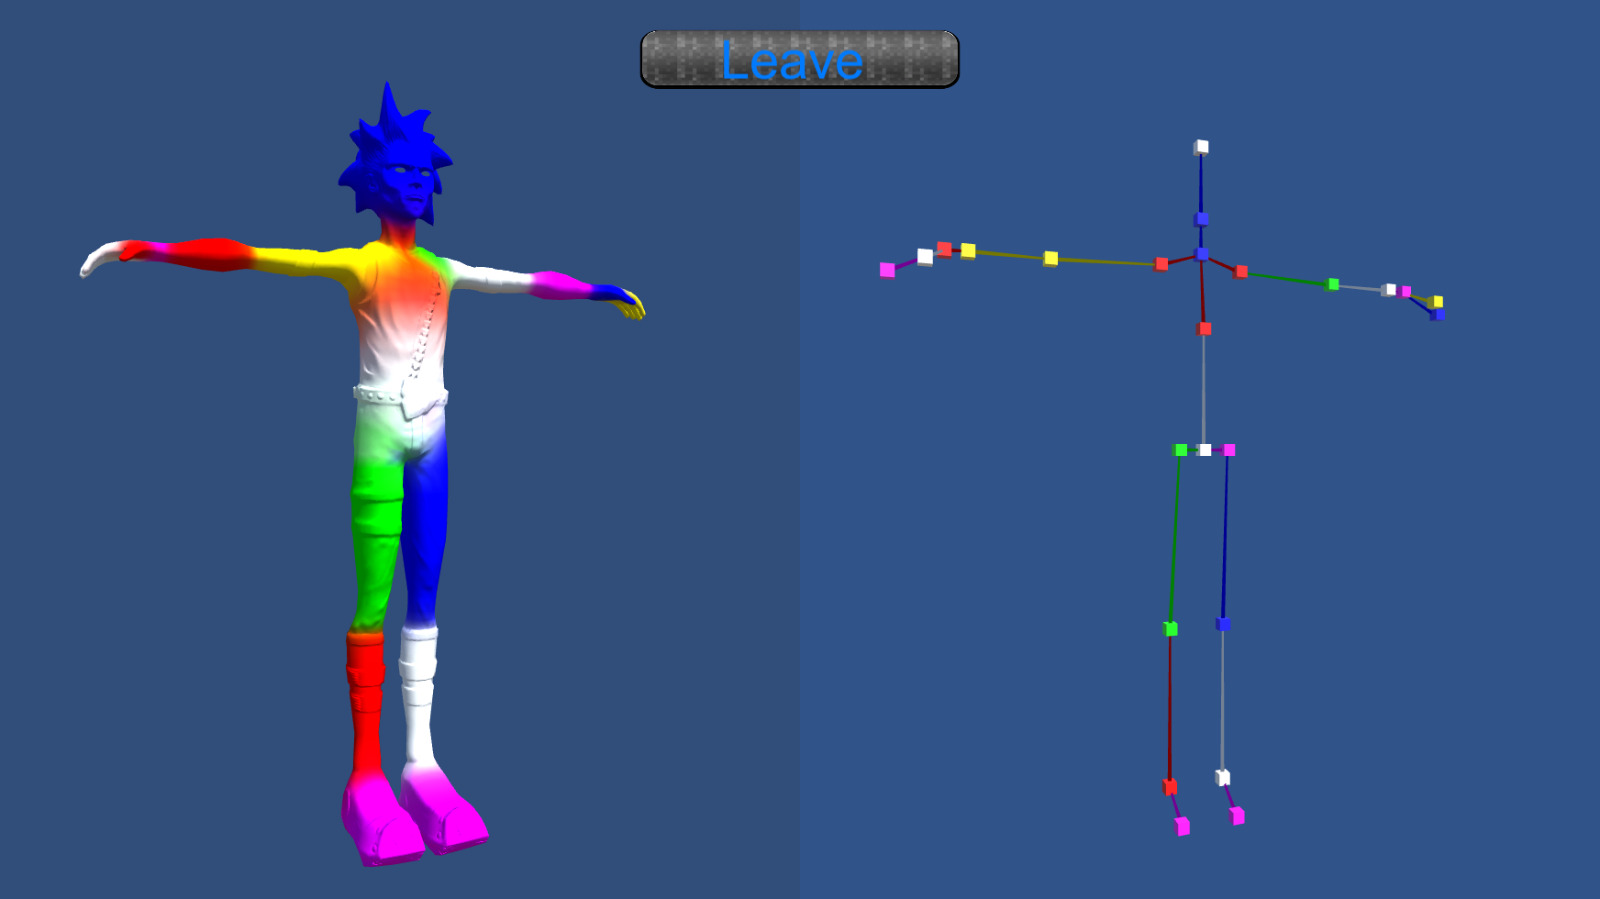
\includegraphics[width=800px]{resting_pose}
		%\begin{flushleft}
		%\begin{center}
		%\textit{Figure 3: Resting pose}
		%\end{center}
		%\end{flushleft}
		%\end{center}
		
%		\begin{figure}[h]
%			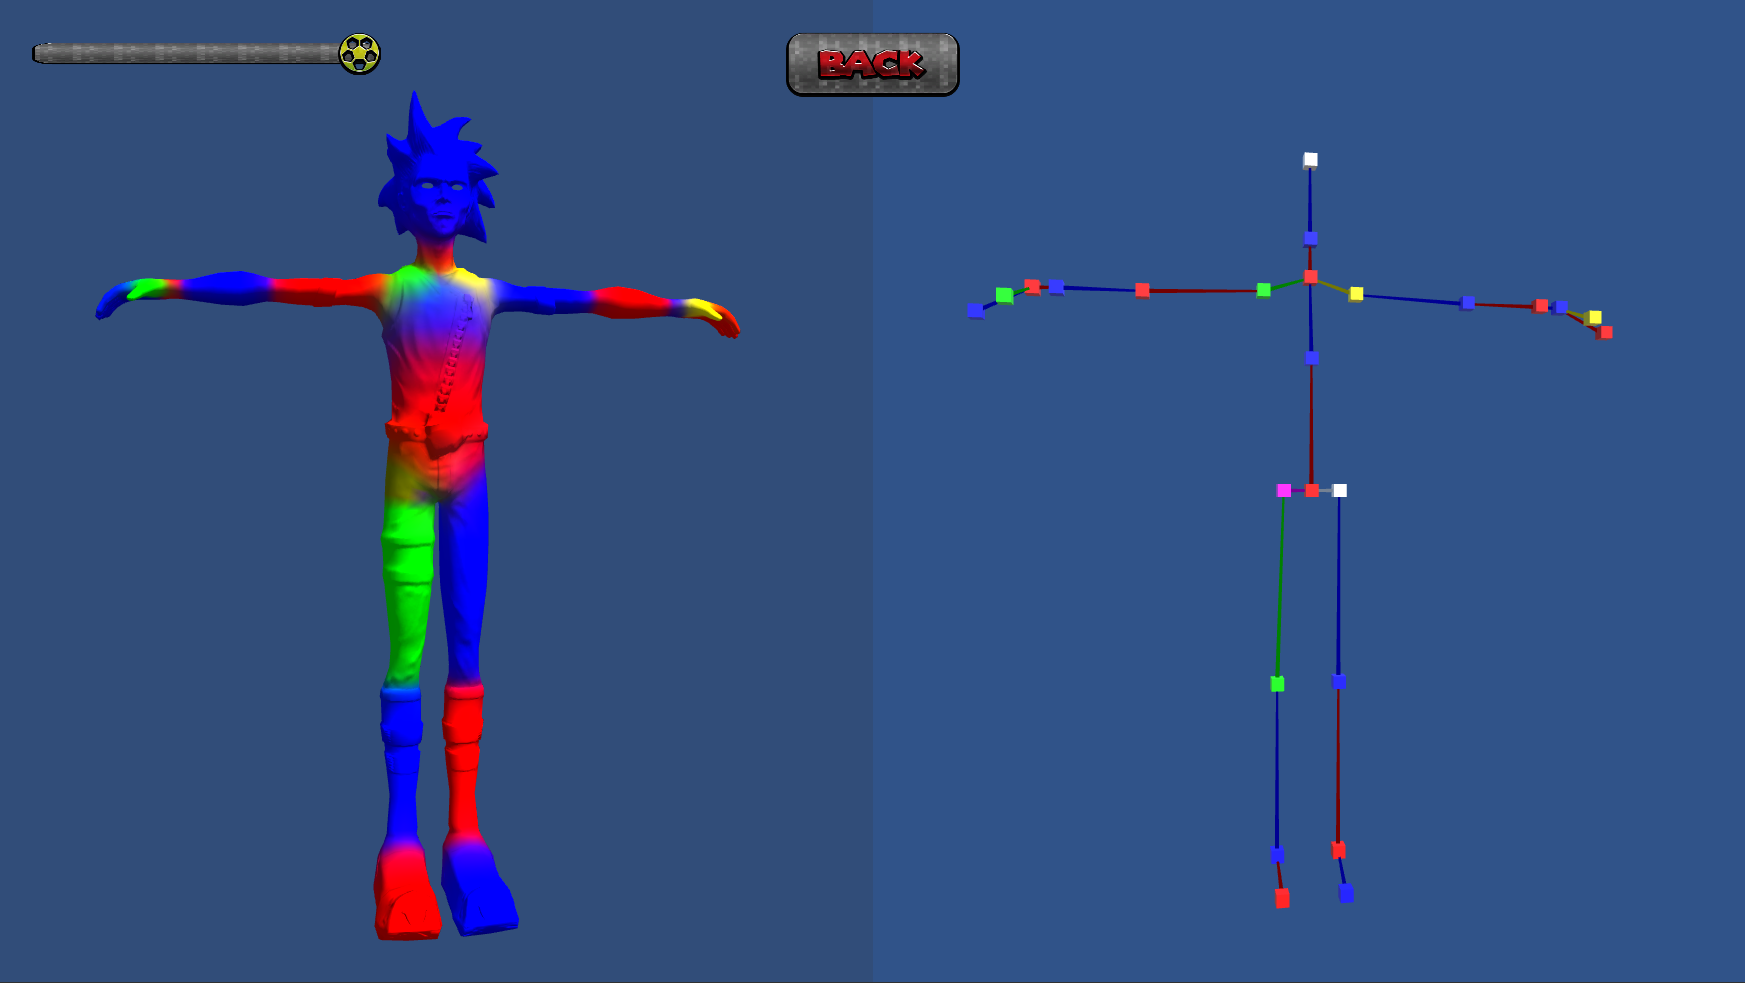
\includegraphics[width=800px]{../Screenshots/weight_colors}
%			\caption{Body weights joints applied to the skeleton and player figure}
%		\end{figure}
	}
}


%%\block{Implementation}{
%The setup 
%}
%
%\block{Optimizations}{
%- Hitboxes around the feet to accurately hit the ball
%}
%}

\column{0.5}{
	\block{\kk}{
		A \textit{Microsoft Kinect Sensor} is used to track the player and his movements. From the raw RGB-D input data a body skeleton is calculated and extracted.
		%
		\image{../Screenshots/weight_colors_cropped.png}{Figure 4: The rest pose mesh and colorful visualized bone weights (left) and the corresponding skeleton bones (right)}{800px}
		%
		By using \linearBlendSkinning{} the rest pose mesh is deformed using the kinematic chain transformations $G(\vec{\omega}_j, j)$. The deformed mesh is assigned to the player game object in a \textit{Unity3D} scene and represents the virtual avatar of the player.\\
		The game content now consists of the player controlling the virtual avatar by moving in front of the \kinect{} and shooting the virtual ball into the holes of the goal wall to score as high as possible.\\
		\image{../Screenshots/main/main_goal.png}{Figure 5: The player shooting onto the goal wall}{800px}
		
%		By 
%		The scene consists of the goal wall and a ball, both which are hittable.
%		Since the implementation of the collision detection and physics calculation are not directly related to this project, we are using Unity's build-in features.
%		Still, the model parameters, the position of the ball relative to the player, the hitbox sizes and shapes as well as the velocity calculation for when the player hits the ball need to be optimized and tuned manually.
%		With this setup, the only thing left is for the player to hit the ball with an appropriate angle and accelerate it towards the goal wall.
		
%		\begin{center}
%		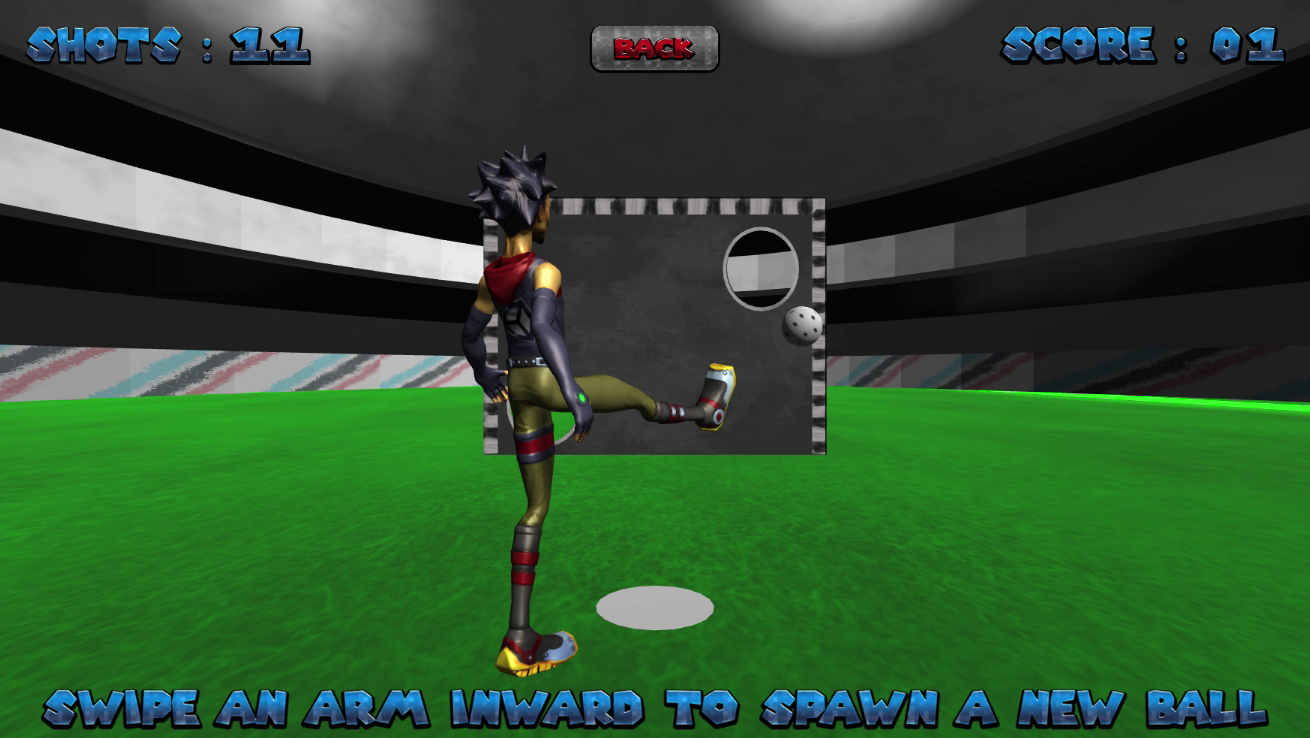
\includegraphics[width=800px]{../Screenshots/main/shooting_scene}
%		\begin{flushleft}
%		\begin{center}
%		\textit{Figure 2: Shooting scene}
%		\end{center}
%		\end{flushleft}
%		\end{center}
	}
	
	\block{Challenges}{
		\subsection*{Ball velocity}
		%
		Calculating the velocity with which the ball is accelerated towards the goal wall must be tuned manually.
		The following aspects account for a realistic value:
		\begin{enumerate}
		  \setlength{\itemsep}{0pt}
		  \item The distance of the player to the goal wall
		  \item The overall scaling of the scene
		  \item The size of the ball in relation to the player
		  \item The amount of hitboxes around the players feet as well as their shape
		  \item The angle of the hit and the rapidity of the body movement when swinging the foot
		  \item The mass of the ball and the foot
		\end{enumerate}
		The first four aspects can be tuned directly in Unity's physics and model framework by modifying the parameters of the models and rigid bodies.
		For the fifth and sixth aspect, applying the formula of an elastic collision yielded very good results:
		\begin{equation}
			v_{ball;shot} = \frac{(2 \cdot m_{\text{ball}} \cdot v_{\text{ball}} + (m_{\text{foot}} - m_{\text{ball}}) \cdot v_{\text{foot}})}{(m_{\text{ball}} + m_{\text{foot}})}
		\end{equation}
		%
		\subsection*{Synchronization}
		%
		The biggest challenge was to synchronize the \kinectSDK{} with \textit{Unity3D}.
		The \kinect{} is recording an RGB-D input stream and through the \kinectSDK{} it provides the joints of the body (25 joints in total) and some orientations.\\
		Even though, ultimately, these values are correct, the joints and rotations do not follow standard character rigging conventions.
		We had to implement a very tough mapping from the received \kinect{} joint data to our rigged character to be able to apply the \linearBlendSkinning{} algorithm presented earlier.\\
		Unfortunately we were not able to integrate correct per bone rotations but could implement the game using some \textit{Unity3D} packages.
	}
}

\end{columns}

\bibliographystyle{plain} 
%\bibliography{references}         


\end{document}
